% !TEX root = ../../../main.tex
% 来源：高中物理甲种本·第三册（电磁·光学·近代物理）
% 章节：课外实验活动 / 测定凹透镜的焦距
% 原始文件：APP2.tex，行 120-136
% 类型：tikz
% ---
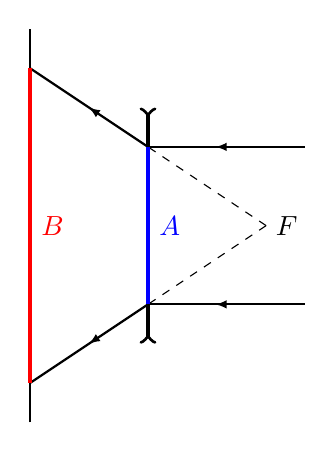
\begin{tikzpicture}[yscale=1]
    \draw[>-<, very thick ] (0,1.5)--(0,-1.5);
\draw[thick] (0,1)--(2,1);
\draw[thick] (0,-1)--(2,-1);
\draw[>=latex, -<] (0,1)--(1,1);
\draw[>=latex, -<]  (0,-1)--(1,-1);

\draw[>=latex, ->] (0,1)--(-1.5/2,1.5);
\draw[>=latex, ->]  (0,-1)--(-1.5/2,-1.5);
\draw[dashed] (1.5,0)node[right]{$F$}--(0,1);
\draw[dashed] (1.5,0)--(0,-1);
\draw[thick] (0,1)--(-1.5,2);
\draw[thick] (0,-1)--(-1.5,-2);
\draw[thick] (-1.5,-2.5)--(-1.5,2.5);
\draw [ultra thick, color=red] (-1.5,2)--node[right]{$B$}(-1.5,-2);
\draw [ultra thick, color=blue] (0,1)--node[right]{$A$}(0,-1);
\end{tikzpicture}
